\titleformat{\chapter}[display]
  {\normalfont\Large\bfseries}
  {\centering Приложение\ \thechapter}
  {0pt}{\Large\centering}
\renewcommand{\thechapter}{\Asbuk{chapter}}

\chapter{Функционально-структурные модели}
\addcontentsline{toc}{chapter}{Приложение А Функционально-структурные модели}
\label{app-fsm}

\pagebreak

\begin{landscape}

	\begin{figure}[t!]
	      \centering
	      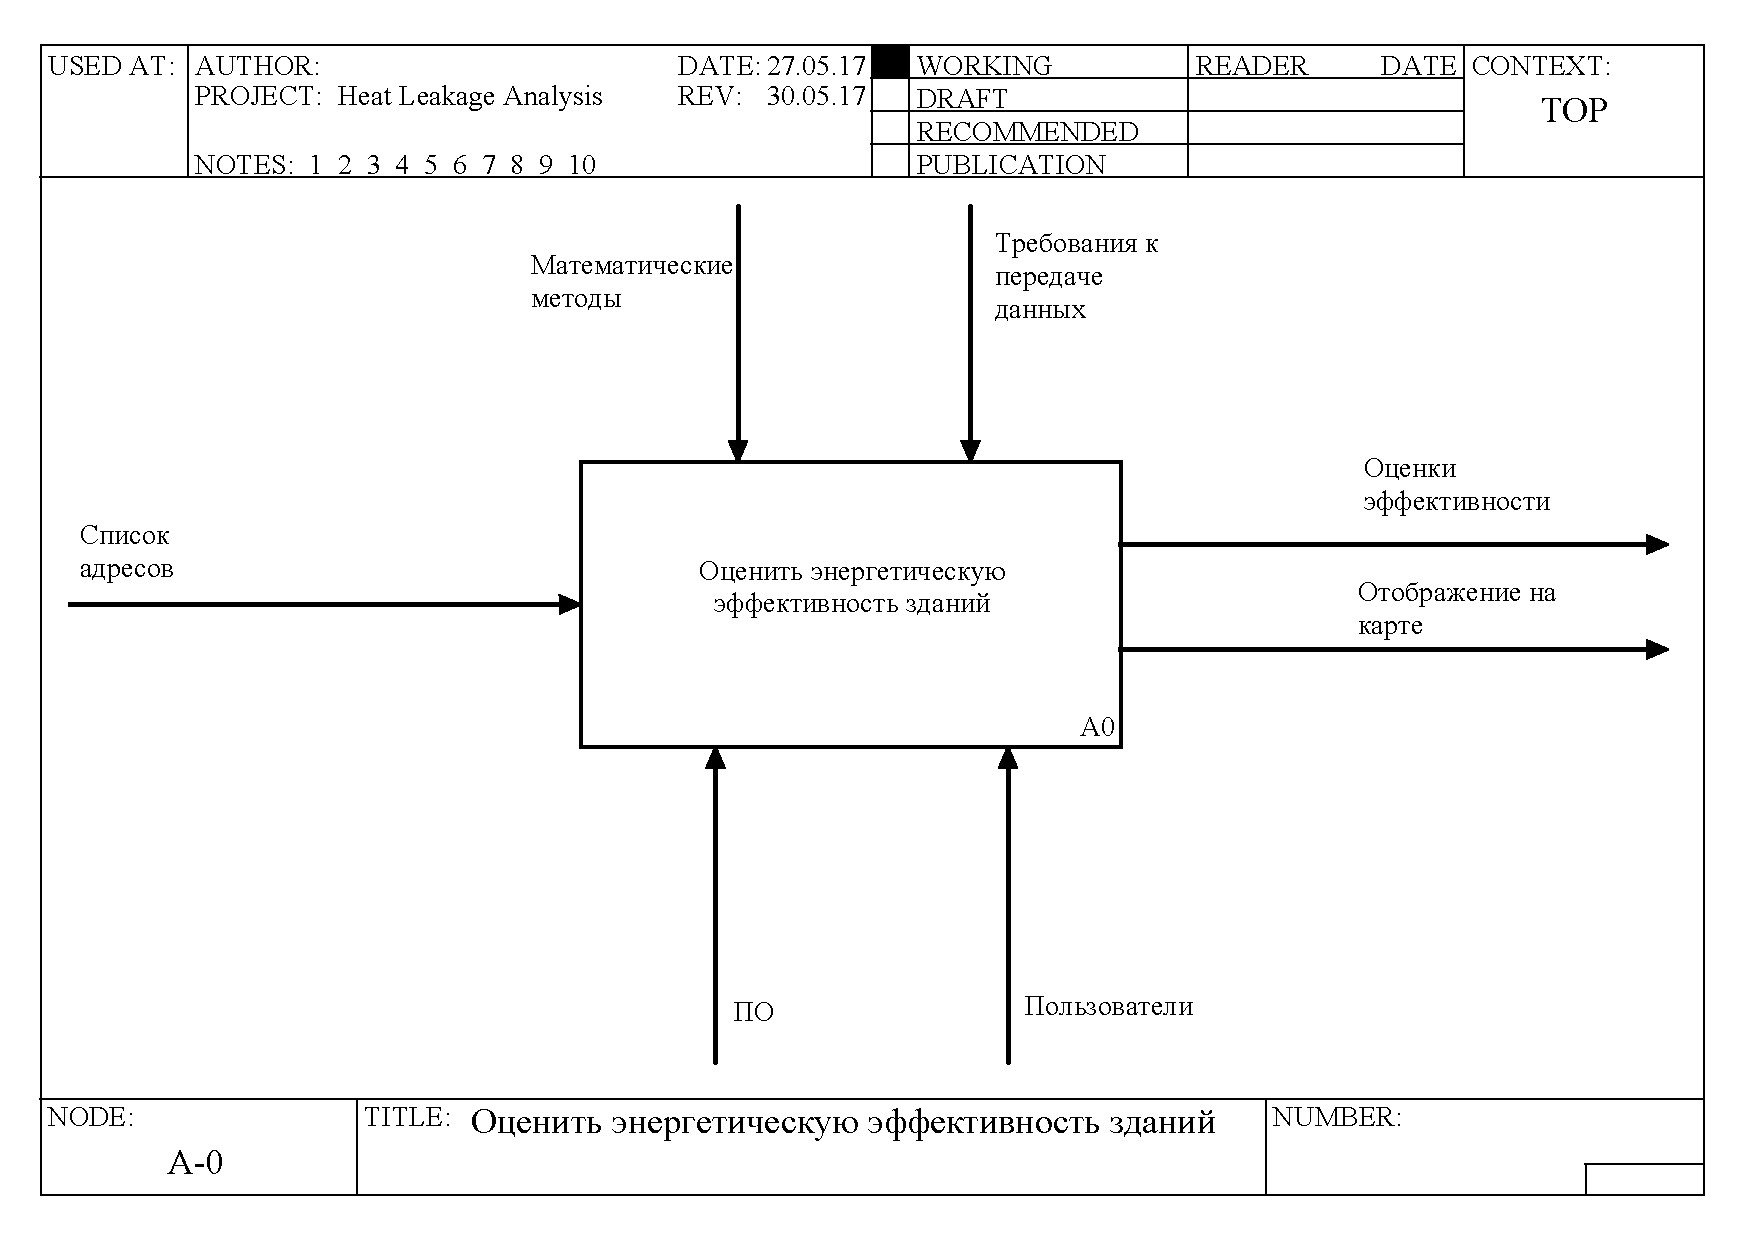
\includegraphics[width=1.3\textwidth]{images/fsm/0}
	      \caption{Контекстная диаграмма функционально-структурной модели предлагаемого решения}
	      \label{fsm:0}
	\end{figure}

\end{landscape}

\pagebreak

\begin{landscape}

	\begin{figure}[t!]
	      \centering
	      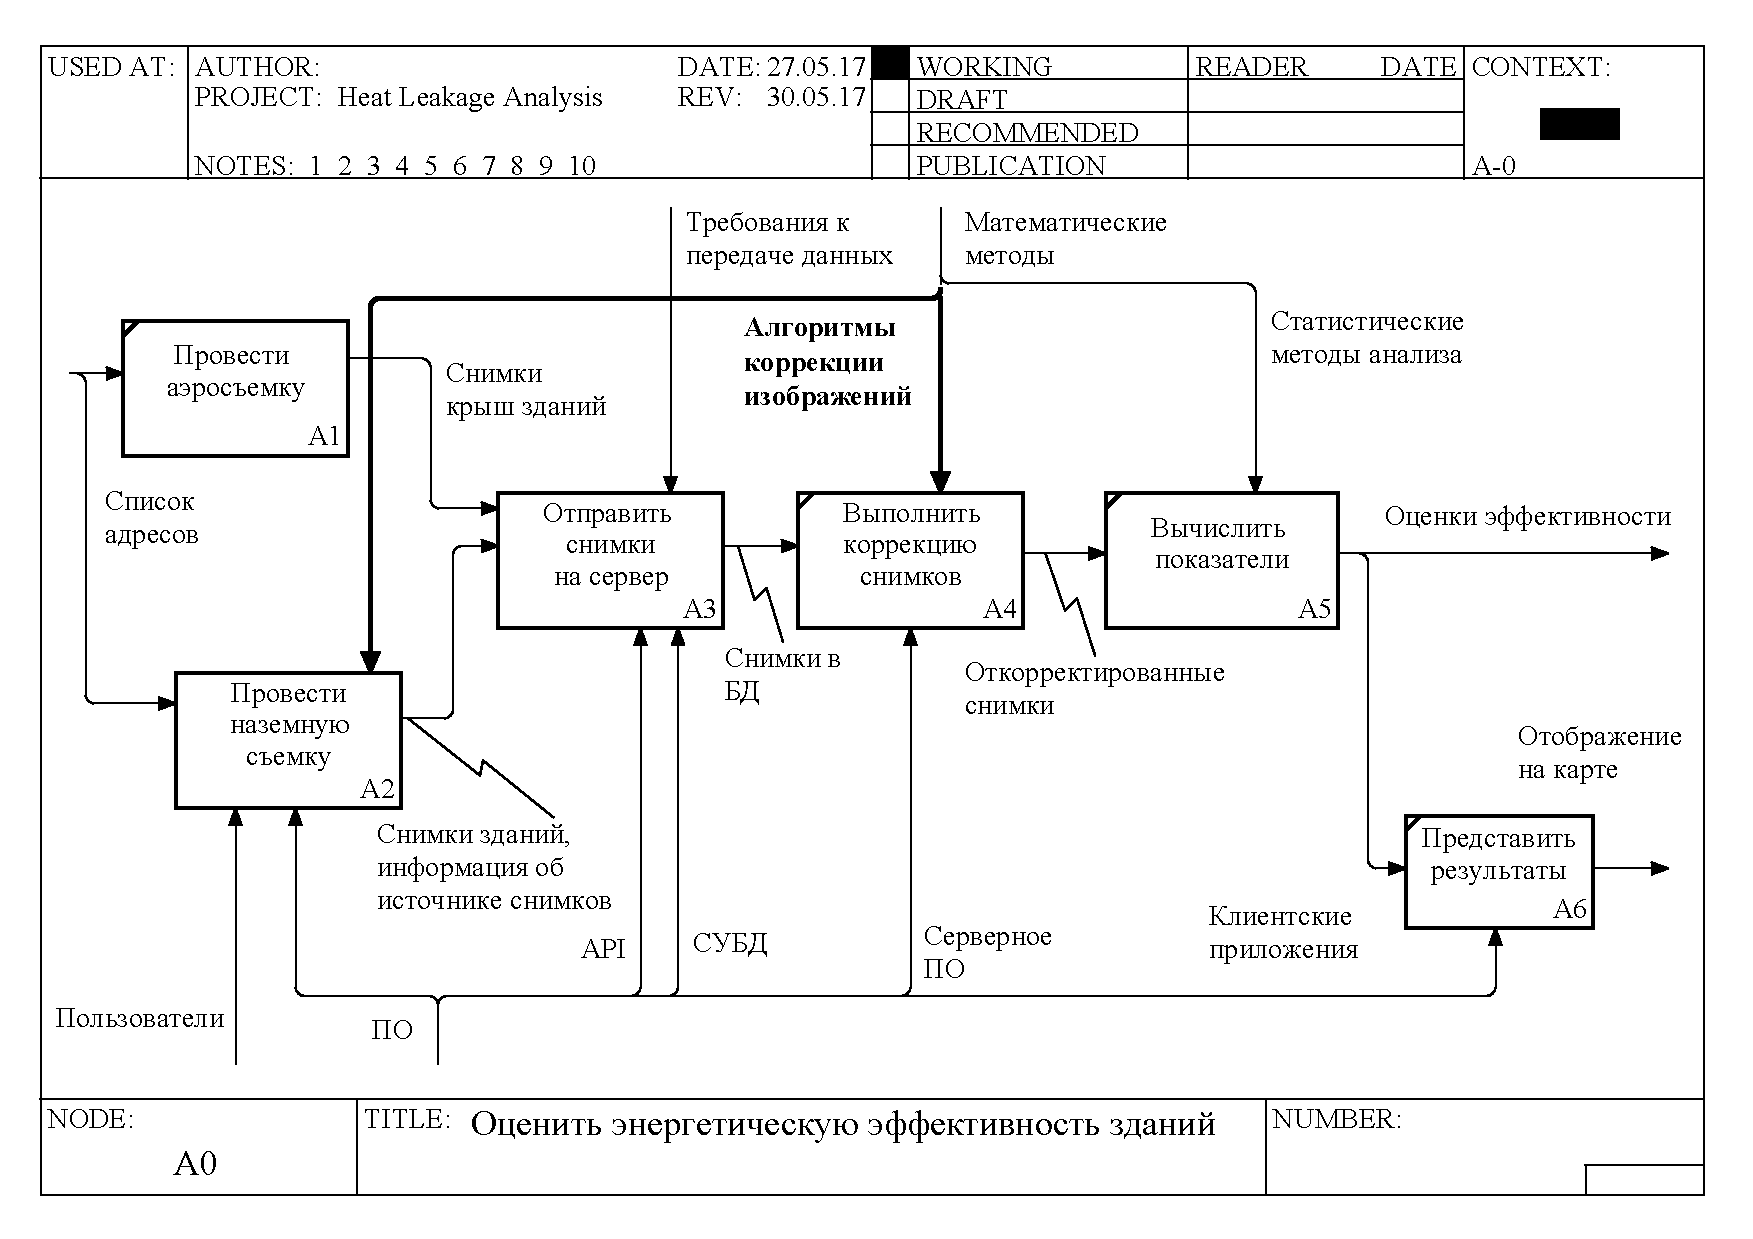
\includegraphics[width=1.3\textwidth]{images/fsm/1}
	      \caption{Диаграмма декомпозиции 1 уровня функционально-структурной модели предлагаемого решения}
	      \label{fsm:1}
	\end{figure}

\end{landscape}

\pagebreak

\begin{landscape}

	\begin{figure}[h!]
	      \centering
	      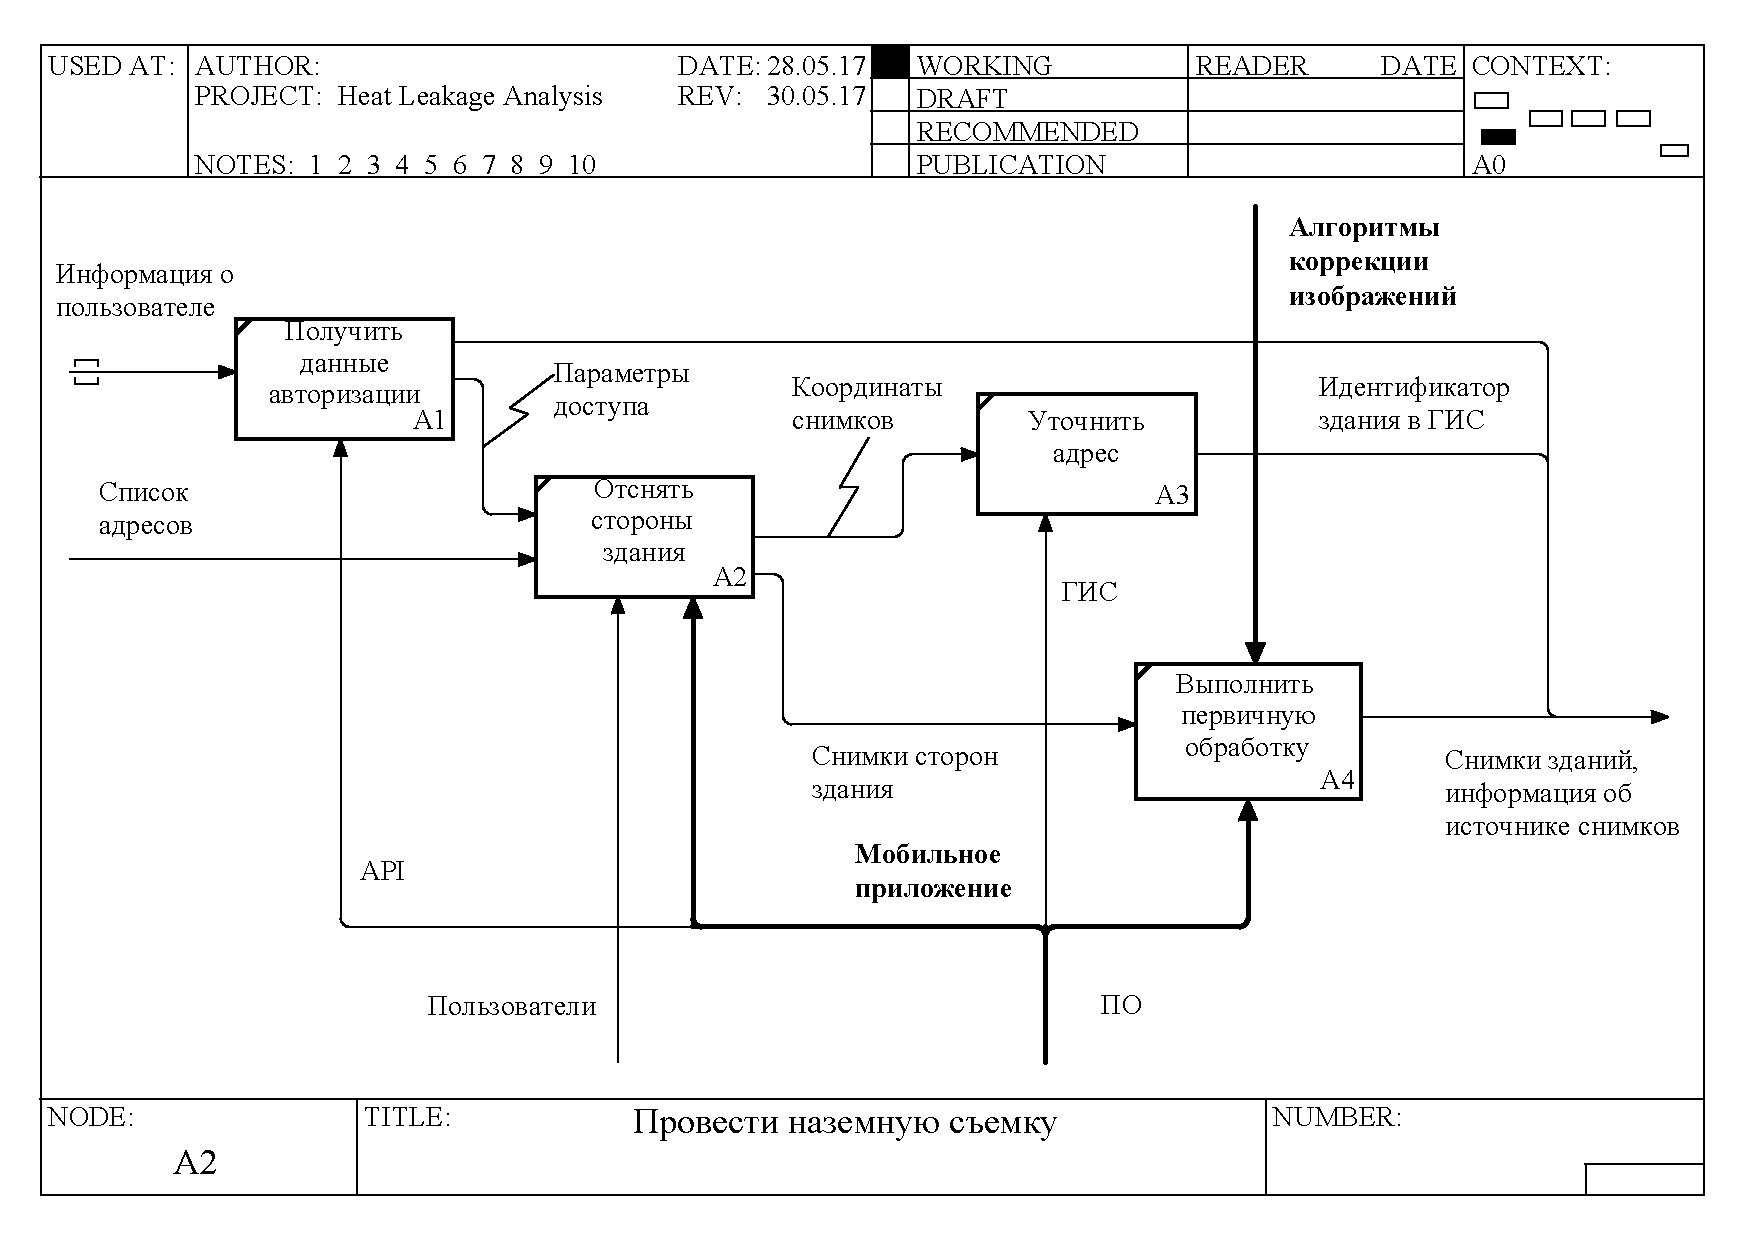
\includegraphics[width=1.3\textwidth]{images/fsm/2}
	      \caption{Диаграмма декомпозиции блока A3 функционально-структурной модели предлагаемого решения}
	      \label{fsm:2}
	\end{figure}

\end{landscape}